%%%%%%%%%%%%%%%%%%%%%%%%%%%%%%%%%%%%%%%%%%%%%%%%%%%%%%%%%%%%%%%%%%%%%%%%%%%%%%%%%%%%%%%%%%%%%%%%%%%
%%%%%%%%%%%%%%%%%%%%%%%%%%%%%%%%%%%%%%%%%%%%%%%%%%%%%%%%%%%%%%%%%%%%%%%%%%%%%%%%%%%%%%%%%%%%%%%%%%%
\chapter{Metodolog\'ia}

%El presente trabajo se llev\'o a cabo \textit{a posteriori}, usando los datos obtenidos en un 
%estudio previo \cite[V\'azquez Tagle, 2016]{VazquezTagle16}; 
%se espera que los resultados encontrados sean una
%extensi\'on de los resultados hallados previamente. 
En esta secci\'on se cita la metodolog\'ia 
manejada en \cite{VazquezTagle16}, 
siendo que el presente trabajo es una extensi\'on de aquel y que parte de los registros obtenidos;
debido a que la naturaleza y origen de estos datos es crucial para el trabajo presente, se trata de
presentar la metodolog\'ia original de la manera m\'as fiel posible.
%, por respeto a los autores y debido a su relevancia en el 
%reciente ana\'alisis sobre los mismos datos. 
Posteriormente se describen los an\'alisis realizados
sobre los datos, a nivel de implementaci\'on, usando el software estad\'istico R
y el paquete \texttt{fractal} \cite{R_citar,R_fractal};
las bases de estos an\'alisis se exponene en secciones anteriores.

En la primera etapa del tarbajo de \cite{VazquezTagle16},
los individuos se sometieron voluntariamente a una bater\'ia de pruebas
neuropsicol\'ogicas para diagnosticar PDC y depresi\'on geri\'atrica (ver m\'as adelante), 
que a su vez fungieron como criterios de
inclusi\'on para una segunda fase del estudio.
En el presente trabajo se han analizado sujetos que fueron excluidos de la segunda etapa de aqu\'el
trabajo, pero que accedieron a participar en la misma; esto se ha hecho con el fin de
verificar si los datos recabados justifican esta restricci\'on en futuros estudios.

En la etapa posterior, los individuos se sometieron voluntariamente a un estudio de la
actividad el\'ectrica cerebral durante el
sue\~no; se realizaron
registros de EEG en 22 sitios de muestreo, adicionalmente se midi\'o
actividad ocular y muscular a trav\'es de EOG y EMG --respectivamente-- con
el fin de detectar adecuadamente las etapas cl\'inicas del sue\~no\cite{AASM07}.
El registro simult\'aneo de estas se\~nales durante el sue\~no recibe el nombre de PSG.

%%%%%%%%%%%%%%%%%%%%%%%%%%%%%%%%%%%%%%%%%%%%%%%%%%%%%%%%%%%%%%%%%%%%%%%%%%%%%%%%%%%%%%%%%%%%%%%%%%%

\section{Pruebas sobre deterioro cognitivo}

La calidad de 'deterioro cognitivo' y 'depresi\'on geri\'atrica' en los participantes fue
determinada a partir de la aplicaci\'on de una pila de pruebas neuropsicol\'ogicas, que se
listan a continuaci\'on.

\begin{itemize}

\item {Evaluaci\'on Neuropsicol\'ogica (Neuropsi)} \cite{Solis03}
%El esquema está constituido por reactivos sencillos y cortos. 
%En la medida de lo posible se incluyeron pruebas con alta validez neuropsicológica y/o se 
%adaptaron estas pruebas para poder evaluar poblaciones de ancianos o psiqui\'atricas. 
%Las \'areas cognoscitivas que eval\'ua 
%el instrumento son 
%\begin{itemize}
%\item[I.] Orientaci\'on
%\item[II.] Atenci\'on y concentraci\'on
%\begin{itemize}
%\item[(a)] Deficiencias en el nivel de conciencia o estado de activaci\'on
%\item[(b)] Atenci\'on selectiva
%\item[(c)] Atenci\'on sostenida
%\item[(d)] Control atencional
%\end{itemize}
%\item[III.] Memoria
%\begin{itemize}
%\item[(a)] Memoria sensorial
%\item[(b)] Memoria a corto plazo
%\item[(c)] Memoria a largo plazo
%\item[(d)] Memoria de trabajo
%\end{itemize}
%\end{itemize}

\item {Mini Mental State Examination (MMSE)} 
%Creado en 1975 como instrumento para 
%la evaluación breve del estado mental, es el test m\'as utilizado para la evaluación cognitiva 
%estandarizada en el \'ambito cl\'inico, sobre todo en el anciano. Es el que dispone de m\'as 
%datos para el cribado, estadiaje y seguimiento de las demencias. As\'i mismo permite detectar 
%alteraciones cognitivas sutiles en pacientes con demencia incipiente o alteraci\'on cognitiva 
%leve, adem\'as de establecer un perfil cognitivo de los diferentes subtipos de 
%demencias.
\cite{Velasco15}

\item {Escala breve para la detecci\'on de ansiedad del anciano (SATS)} 
%Es un instrumento 
%que 
%consta de 10 preguntas espec\'ificas sobre malestar psicol\'ogico que se refieren a los 
%s\'intomas de ansiedad que puede tener una persona durante las cuatro semanas previas a la 
%aplicaci\'on. Las opciones de respuesta de las preguntas son tipo Likert, categorizadas en una 
%escala ordinal de cinco niveles: siempre, casi siempre, a veces, casi nunca y nunca. 
%A la respuesta \textit{nunca} se le asigna el valor escalar de 1 y a la respuesta 
%\textit{siempre}, de 5 puntos. La suma de las puntaciones tiene un m\'inimo de 10 y un máximo de 
%50. Los rangos del instrumento presentan cuatro niveles: bajo (10–15), moderado (16–21), 
%alto (22–29), y muy alto (30–50). La consistencia interna del instrumento fue de $\alpha$=0.90
\cite{Vargas11}

\item {Escala sobre las actividades cotidianas de la vida diaria (KATZ)} 
%Eval\'ua el nivel
%de independencia de las actividades de la vida diaria en pacientes con deterioro cognoscitivo y 
%demencia. Su aplicaci\'on es de alrededor de diez a quince minutos y no requiere de capacitaci\'on 
%previa. Consta de una primera parte donde se consignan los datos del paciente y del informante, 
%lugar, fecha y nombre del evaluador. Una segunda parte, est\'a formada por nueve \'items que se 
%corresponden con las actividades de la vida diaria b\'asicas (continencia urinaria, continencia 
%fecal, aseo, toilette, alimentaci\'on, movilidad, traslado dentro y fuera del hogar, ba\~no y 
%vestido), a su vez cada una de ellas est\'a desglosada en las acciones que conforman la tarea y la 
%forma en que el paciente la lleva a cabo. A cada actividad le corresponde un puntaje parcial, que 
%refleja la capacidad funcional del paciente. Se debe tener en cuenta que el \'item se corresponde 
%con el nivel \'optimo de funcionamiento y le corresponde el puntaje m\'as alto dentro de la escala,
%6 puntos. La suma de todos los resultados sirve para arribar a un puntaje total, que se 
%correlaciona con uno de los siete niveles de desempe\~no, determinando cu\'ando una persona 
%requiere indicaci\'on, supervisi\'on o asistencia f\'isica/verbal de otra para ejecutar todos los 
%pasos de una actividad. El puntaje total es 60 puntos, que corresponde al desempe\~no 
%independiente.
\cite{Roumec14}

\item {Escala de Depresi\'on Geri\'atrica (Gds)} 
%Esta escala ha sido probada y usada 
%extensamente 
%en la población adulta mayor. Con la escala Gds se valora la depresión en el adulto mayor que 
%puede confundirse con el deterioro cognitivo. Es conocido que la depresi\'on puede disparar el 
%deterioro f\'isico, cognitivo y social particularmente en el adulto 
%mayor. 
\cite{Greenberg12,Cuijpers13}

\end{itemize}

%%%%%%%%%%%%%%%%%%%%%%%%%%%%%%%%%%%%%%%%%%%%%%%%%%%%%%%%%%%%%%%%%%%%%%%%%%%%%%%%%%%%%%%%%%%%%%%%%%%

\section{Participantes}

En el trabajo original,
la muestra se eligi\'o de una manera no probabilística de sujetos tipo \cite{Garcia09}. De aquellos
s\'olo se han considerado 11 sujetos que accedieron a la segunda fase del estudio (obtenci\'on
de registros de PSG), que en conjunto conforman una muestra no necesariamente respresentativa de
la muestra total.

Usando los reultados de la bater\'ia de pruebas neuropsicol\'ogicas, los sujetos se dividieron
en tres grupos: PDC, Normal y Extra (aquellos no considerados en el estudio original). En la tabla
\ref{tab_sujetos} se han concentrado estos resultados.

\begin{table}
\centering
\begin{tabular}{l|ccc|ccccc|c}
%\hline 
%Nombre & Sexo & Edad & Esc. & Neuropsi & MMSE & SATS & KATZ & Gds & Notas \\
\textbf{Nombre} & \textbf{Sexo} & \textbf{Edad} & \textbf{Esc.} & \textbf{Neuropsi} & \textbf{MMSE} & \textbf{SATS} & \textbf{KATZ} & \textbf{Gds} & \textbf{Notas} \\
\hline 
VCR    & F    & 59   & 12   & 107      & 29   & 21   & 0    & 3 & \\
MJH    & F    & 72   & 9    & 113      & 30   & 18   & 0    & 0 & \\
JAE    & F    & 78   & 5    & 102      & 28   & 19   & 0    & 5 & \\
GHA    & M    & 65   & 9    & 107.5    & 30   & 23   & 0    & 7 & Disminuci\'on aguda visual y auditiva, alcoholismo previo \\
MFGR   & F    & 67   & 11   & 110      & 30   & 18   & 0  &  \\
\hline 
CLO    & F    & 68   & 5    & 81       & 28 & 22 & 1 & 6 &  \\
RLO    & F    & 63   & 9    & 90       & 29 & 20 & 0 & 3 &  \\
RRU    & M    & 69   & 9    & 85       & 27 & 10 & 0 & 3 &  \\
JGZ    & M    & 65   & 11   & 87       & 25 & 20 & 0 & 1 &  \\
\hline 
FGH    & M    & 71   & 9    & 83.5     & 21 & 23 & 0 & 4  &  Par\'alisis facial, hipotiroides, columna, cataratas  \\
MGG    & F    & 61   & 9    & 114      & 28 & 29 & 1 & 14 &  \\
EMT    & M    & 50   & 22   & 106      & 30 & 15 & 0 & 4  &  \\
%\hline 
\end{tabular} 
\label{tab_sujetos}
\caption{Resultados de las pruebas neuropsicol\'ogicas aplicadas a los sujetos considerados
en este trabajo, adem\'as de algunos datos generales de estos mismos sujetos}
\end{table}


En el protocolo para la obtenci\'on de estos datos en \cite{VazquezTagle16} 
se declara la participaci\'on informada 
y libre de los sujetos bajo los siguientes t\'erminos:
\begin{quote}
La participaci\'on en el estudio es completamente 
voluntaria, pudiendo los sujetos abandonar las intervenciones en cualquier momento. Todos los 
participantes firmaron un consentimiento informado previamente a su inclusi\'on en el estudio. 
Los protocolos experimentales empleados en esta investigaci\'on fueron previamente aprobados por 
el Comit\'e \'Etico de Investigaci\'on en humanos de la Universidad Autónoma del Estado de Hidalgo.
%La muestra se eligi\'o de una manera no probabilística de sujetos tipo \cite{Garcia09}.
\end{quote}

%%%%%%%%%%%%%%%%%%%%%%%%%%%%%%%%%%%%%%%%%%%%%%%%%%%%%%%%%%%%%%%%%%%%%%%%%%%%%%%%%%%%%%%%%%%%%%%%%%%

\section{Electroencefal\'ografo utilizado}

Para registrar el PSG se ha usado 
{electroencefal\'ografo digital MEDICID 5.} 
(Neuronic mexicana S.A. de C.V.);
% MEDICID. MEDICID 5. 2016; : 1.]
%Es un electroencefal\'ografo digital de 
cuenta con
32 canales, 24 de ellos monopolares con posibilidades de 
programaci\'on y 8 bipolares con la posibilidad de conexi\'on monopolar para conformar 32 canales 
con referencia com\'un. 
%Esto hace posible preparar por software los montajes que comunmente son 
%conocidos en los equipos tradicionales de poligraf\'ia en papel. 
%Los amplificadores bipolares son 
%especialmente dise\~nados para la conexi\'on sensorial o la transducci\'on de la medici\'on por 
%signos biof\'isicos, (esfuerzo respiratorio abdominal y tor\'acico, flujo a\'ereo nasal y bucal) 
%cuando los registros poligr\'aficos est\'an hechos. 
%%%Con el MEDICID se pueden usar las siguientes aplicaciones: 
%%%\begin{itemize}
%%%\item \underline{Trackwalker.} Sistema b\'asico de electroencefalograf\'ia digital con EEG 
%%%cuantitativo y mapeo cerebral.
%%%
%%%\item \underline{Dream Hunter.} Sistema para estudios del sue\~no.
%%%
%%%\item \underline{Mind Tracer.} Sistema para el estudio de Potenciales Evocados 
%%%relacionados a eventos.
%%%
%%%\item \underline{EP Workstation.} Sistema para la estimaci\'on y el an\'alisis de los 
%%%Potenciales Relacionados a Eventos (PRE) end\'ogenos de alta densidad (128 canales). 
%%%\end{itemize}
Especificaciones T\'ecnicas:
\begin{itemize}
\item 24 canales monopolares (0.05 -- 100 Hz)
\item 8 canales bipolares para poligraf\'ia (0.5 -- 100 Hz)
\item 3 canales de C.C. (0--160 Hz)
\item 1 canal de temperatura (30--40 C)
\item 1 estimulador f\'otico (0.5--33 Hz)
\item Sistema A/D: 16 bits
\item Frec. Muestreo: Hasta 500 Hz (36 canales)
\item Voltaje Alimentaci\'on: 100--240 V, 50/60 Hz
\item Interfaz: USB
\item Dimensiones: Bloque de control: (257x315x55 mm)
\item Peso: Bloque de control: 2.5 kg
\item Bloque amplificadores: (110x187x50 mm)
\item Bloque amplificadores: 1.0 kg
\item Seguridad el\'ectrica: Clase I Tipo BF (Certificado según EN60601-1)
\end{itemize}

%%%%%%%%%%%%%%%%%%%%%%%%%%%%%%%%%%%%%%%%%%%%%%%%%%%%%%%%%%%%%%%%%%%%%%%%%%%%%%%%%%%%%%%%%%%%%%%%%%%

\section{Registro de PSG}

Una vez aplicado el Neuropsi y toda la bater\'ia de pruebas ya mencionada, los adultos mayores
participantes fueron invitados a acudir a las instalaciones de la Cl\'inica Gerontol\'ogica de 
Sue\~no, ubicada en las instalaciones del Instituto de Ciencias de la Salud de la Universidad 
Aut\'onoma del Estado de Hidalgo.

Los participantes recibieron instrucciones de realizar una rutina normal de actividades durante la 
semana que precedi\'o al estudio. Tambi\'en se les recomend\'o que no ingirieran bebidas 
alcoh\'olicas o energizantes como caf\'e o refrescos durante las 24 horas previas al experimento, 
ni durmieran siesta el d\'ia del estudio. 

%Cada participante lleg\'o a las instalaciones alrededor de las 17:00 hrs. para la colocaci\'on de 
%los electrodos, ya que este procedimiento tarda de entre 2 a 3 horas. La hora de comienzo del 
%registro de PSG fue adaptado a la hora habitual de acostarse de cada sujeto.

El protocolo de PSG incluYE 19 electrodos de EEG: 
\begin{itemize}
\item Fp1 
\item Fp2
\item AF7
\item AF3
\item AFz
\item AF4
\item AF8
\item F7
\item F5
\item F3
\item F1
\item Fz
\item F2
\item F4
\item F6
\item F8
\item FT7 
\item FC5
\item FC3
\item FC1
\item FCz
\item FC2
\item FC4
\item FC6
\item FT8
\item T7
\item C5
\item C3
\item C1
\item Cz
\item C2
\item C4
\item C6
\item T8
\item TP7
\item CP5
\item CP3
\item CP1
\item CPz
\item CP2
\item CP4
\item CP6
\item TP8
\item P7
\item P5
\item P3
\item P1
\item Pz
\item P2
\item P4
\item P6
\item P8
\item PO7
\item PO3
\item POz
\item PO4
\item PO8
\item O1
\item O2
\end{itemize}
4 electrodos de EOG para registrar movimientos oculares horizontales y verticales, 
y 2 electrodos de EMG colocados en los m\'usculos submentonianos para registrar la actividad 
muscular. 
La colocaci\'on de los electrodos para registrar la actividad EEG se realiz\'o siguiendo las 
coordenadas del Sistema Internacional 10-20\cite{Coleman87}.

\begin{figure}
\centering
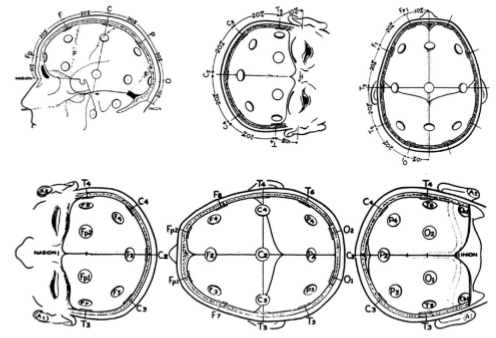
\includegraphics[width=\linewidth]{figura_6.png} 
\caption{El sistema 10--20, recomendado por la
International Federation of EEG Societies. 
%\cite{Jasper58,AASM07}
}
%\label{img1020}
\end{figure}

%Previamente a la colocaci\'on de cada electrodo, se frot\'o la zona de inter\'es con un algod\'on 
%empapado en crema abrasiva con el objetivo de eliminar las c\'elulas muertas y la grasa de la piel.
%Posteriormente, la copa de cada electrodo se rellen\'o con una pasta electrol\'itica 
%conductora (Ten20\texttrademark, Weaver) para mejorar la conductividad  entre la piel y el 
%electrodo. Los electrodos para registrar el EEG se fijaron al cuero cabelludo con colodi\'on 
%(solución al 4\%, Panreac), mientras que los electrodos de poligraf\'ia (EOG y EMG) fueron 
%adheridos a la piel de la cara con cinta quir\'urgica extra-adhesiva (Cinta 
%Micropore\texttrademark). Para acelerar el proceso de fijaci\'on y secado del colodi\'on, se 
%aplic\'o aire comprimido a cada electrodo colocado sobre el cuero cabelludo.

Las se\~nales electrofisiol\'ogicas de cada registro PSG fueron amplificadas, filtradas y 
digitalizadas con el programa para ordenador \texttt{Registro de sue\~no} 
para su posterior interpretaci\'on. 
El registro se llev\'o a cabo con una tasa de muestreo de 500 Hz o 200 Hz (puntos por segundo)
seg\'un la disponibilidad del electroencefal\'ografo.

%%%%%%%%%%%%%%%%%%%%%%%%%%%%%%%%%%%%%%%%%%%%%%%%%%%%%%%%%%%%%%%%%%%%%%%%%%%%%%%%%%%%%%%%%%%%%%%%%%%

\section{Clasificaci\'on de las etapas de sue\~no}

La clasificaci\'on de las diferentes fases del sue\~no en el registro PSG se realiz\'o manualmente 
sobre \'epocas de EEG de 30 segundos (filtro paso de banda de 0.5--30 Hz) siguiendo los criterios 
estandarizados de la AAIC\cite{Hori01}, que se exponen a continuación:
\begin{description}
\item[Vigilia relajada con ojos cerrados] Presencia de ritmo alfa contin\'uo con m\'axima amplitud 
sobre regiones de la corteza parieto-occipital. Tono muscular relativamente alto y ausencia de 
movimientos oculares.

\item[Fase 1] %Transici\'on entre la vigilia y el sue\~no ligero. 
Presencia intermitente de 
actividad alfa en menos del 50\% de la \'epoca junto con movimientos oculares lentos y una ligera 
reducci\'on del tono muscular respecto al de vigilia.

\item[Fase 2] Presencia de complejos K y husos de sue\~no. Puede aparecer hasta un 20\% de ondas 
lentas (ritmo delta, 0.5-3 Hz) en la \'epoca. Ausencia de actividad ocular y tono muscular bajo.

\item[Fase 3] Presencia de ondas lentas con amplitudes superiores a 75 $\mu$V en m\'as del
20\% y menos del 50\% de la \'epoca. Pueden tambi\'en aparecer complejos K y husos de sue\~no de 
forma espor\'adica. Ausencia de actividad ocular y tono muscular bajo.

\item[Fase 4] Presencia de ondas lentas en m\'as del 50\% de la época. Las dem\'as 
caracter\'isticas son similares a las de la fase 3.

\item[Fase MOR] Presencia de actividad EEG de baja amplitud y frecuencias entremezcladas 
(theta-alfa-beta) similar a la observada en el estado de vigilia activa con ojos abiertos.
\end{description}

%%%%%%%%%%%%%%%%%%%%%%%%%%%%%%%%%%%%%%%%%%%%%%%%%%%%%%%%%%%%%%%%%%%%%%%%%%%%%%%%%%%%%%%%%%%%%%%%%%%

\section{Aplicaci\'on del test de Priestley-Subba Rao (PSR)}

Para el an\'alisis de los registros de PSG se us\'o el software estad\'istico R\cite{R_citar}, 
as\'i como el paquete \texttt{fractal} \cite{R_fractal}.

Los registros digitalizados de PSG fueron convertidos a formato de texto (\texttt{.txt}) bajo
la codificaci\'on ASCII, a raz\'on de un archivo por cada canal. Posteriormente fueron importados
en el ambiente R y segmentados en sub-series de 30 segundos [10 segundos para algunos 
registros] acordes al concepto de \'epocas, y tomando en cuenta la tasa de muestreo de 512 [200]
puntos por segundo. 
En una primera etapa del trabajo solamente fueron incluidas sub-series correspondientes a
\'epocas de sue\~no MOR

Como se mencion\'o anteriormente, el test PSR est\'a pensado para
series de tiempo con valor esperado constante 0, y varianza finita en todo momento. Si bien la 
segunda condici\'on se satisface claramente en los sistemas biol\'ogicos [buscar respaldo
para esta afirmaci\'on], la primera condici\'on no tiene por qu\'e cumplirse, de modo que es 
forzada
usando el filtro no-param\'etrico STL\cite{Cleveland1990} sobre cada una de las 
sub-series\footnote{En la secci\'on de discusi\'on se abordar\'an las consecuencias de tal fitrado,
mientras que en un anexo se describen los detalles en s\'i de este filtro.}.


Los detalles te\'oricos del test PSR fueron discutidos con anterioridad. A modo
de resumen: se calcula el logaritmo del m\'odulo de la funci\'on de densidad
espectral para algunos puntos en el tiempo y las frecuencias, para lo cual se usa un estimador
local cuya varianza es conocida; posteriormente se procede a probar, como prueba de
hip\'otesis, que las cantidades obtenidas anteriormente son estad\'isticamente constantes
en el tiempo.
Este test se encuentra implementado en R bajo la funci\'on \texttt{stationarity}
del paquete \texttt{fractal}; en la figura \ref{res_psr} puede verse la forma en que se
visualizan los resultados.

\begin{figure}
\centering
\begin{lstlisting}
Priestley-Subba Rao stationarity Test for datos
-----------------------------------------------
Samples used              : 3072 
Samples available         : 3069 
Sampling interval         : 1 
SDF estimator             : Multitaper 
  Number of (sine) tapers : 5 
  Centered                : TRUE 
  Recentered              : FALSE 
Number of blocks          : 11 
Block size                : 279 
Number of blocks          : 11 
p-value for T             : 0.4130131 
p-value for I+R           : 0.1787949 
p-value for T+I+R         : 0.1801353 
\end{lstlisting}
\caption{Resultado de una ejecuci\'on t\'ipica de la funci\'on \texttt{stationarity}. 
El n\'umero de bloques \texttt{n.blocks} define la cantidad de puntos en el tiempo
para los cuales se calcular\'a el estimador de la funci\'on de densidad espectral (SDF),
se calcula por default como
$\max \left( 2 , \left\lfloor \log_2\left( N \right) \right\rfloor \right)$, donde
$N$ es la cantidad de datos en la serie, aunque puede ingresarse un valor arbitrario.
Los filtros \textit{tapers} son usados para compensar el efecto de frecuencias m\'as altas que la 
tasa de muestreo, o de aquellas cuya longitud de onda sea mayor que la longitud de la serie;
para mayor informaci\'on vea la ssecci\'on [?].
Cabe se\~nalar el antepen\'ultimo rengl\'on (\texttt{p-value for T}), que refleja el rechazo de 
la prueba de 
hip\'otesis de estacionariedad.}
\label{res_psr}
\end{figure}

%\begin{tabular}{cc}
%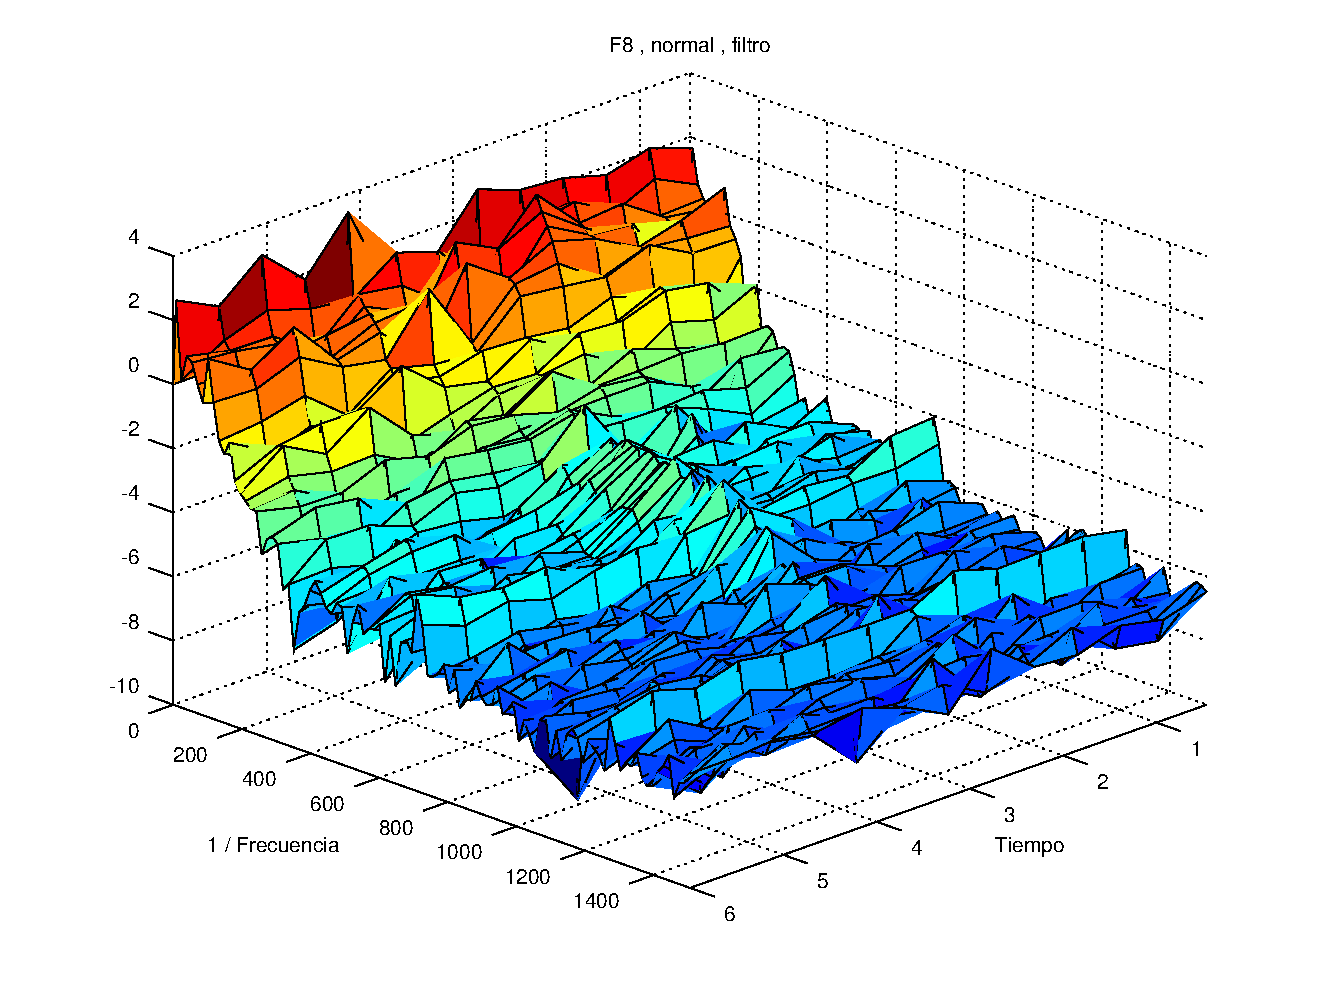
\includegraphics[width=0.5\linewidth]{n8f.pdf} 
%&
%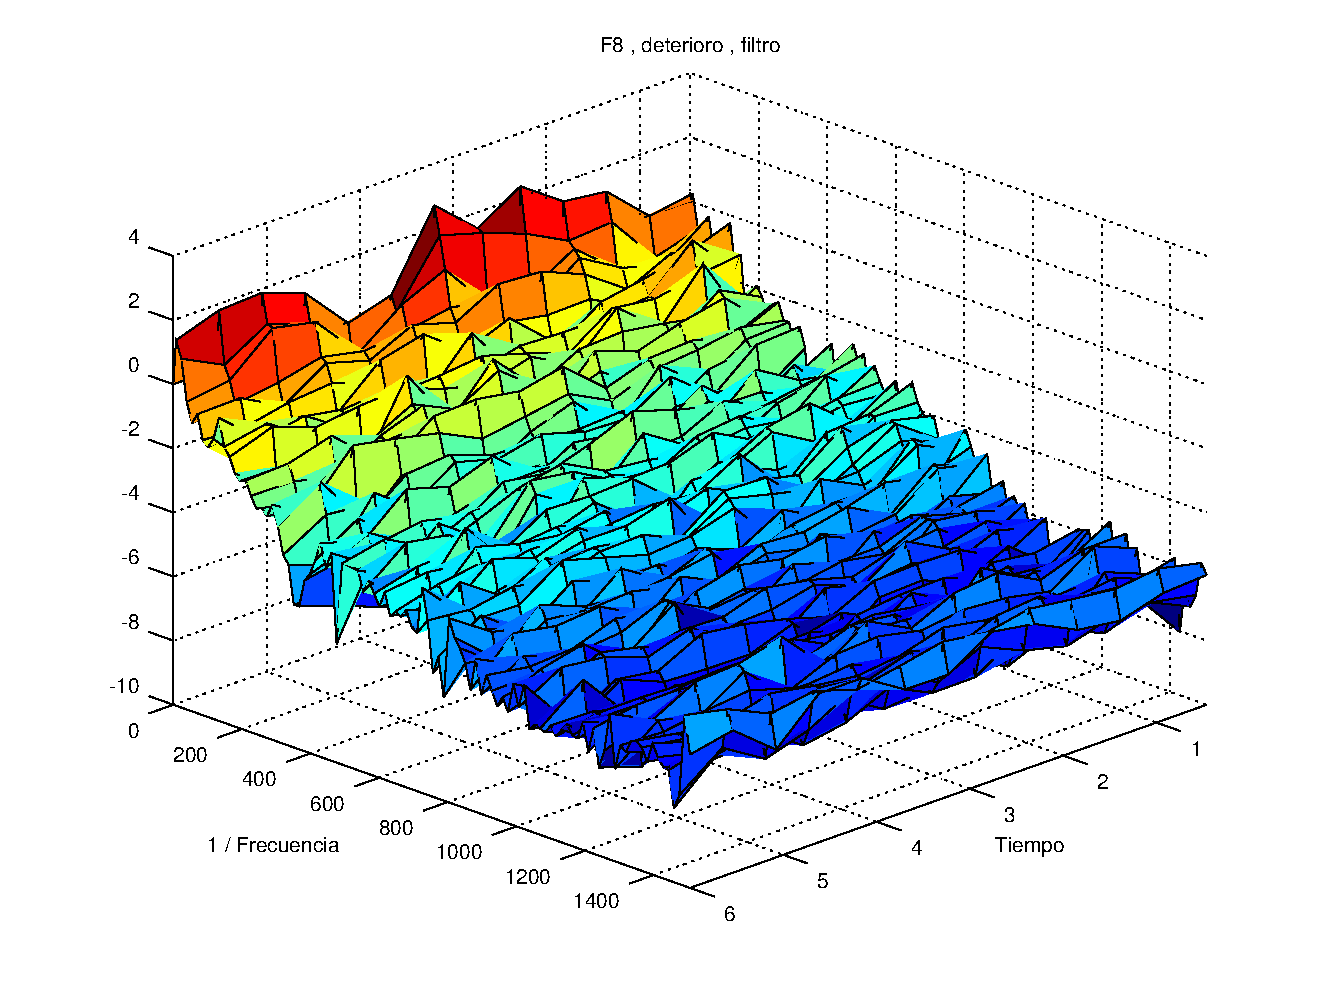
\includegraphics[width=0.5\linewidth]{d8f.pdf} 
%\\
%\begin{lstlisting}
%T      : 0 
%I+R    : 5.787895e-09 
%T+I+R  : 0 
%\end{lstlisting}
%&
%\begin{lstlisting}
%T      : 0.00332259 
%I+R    : 0.03502537 
%T+I+R  : 0.01598073 
%\end{lstlisting}
%\end{tabular}

%Este test se ha realizado para TODAS las epocas disponibles, pero como el test
%es r\'apido s\'olo ha tardado 1 hora por sujeto usando una maquina potente [debo citar
%los detalles tecnicos, y la cantidad de puntos procesados. Segun Nason (2012), el test PSR
%tiene una velocidad del orden de $N log(N)$, con $N$ la cantidad de puntos procesados, y 
%con lo cual es bastante mas rapido que otras pruebas].

Una vez se hubo realizado el test para todas las \'epocas consideradas, se dispuso de los 
resultados de manera gr\'afica  como se muestra en las figuras \ref{ejemplo1}.
Por cada canal de PSG (EEG, EOG y EMG), se colocan en l\'inea horizontal un cuadro por cada
\'epoca en blanco o negro seg\'un el segmento referido haya sido clasificado como
no-estacionario o posiblemente estacionario; posteriormente se han colocado verticalmente las
l\'ineas as\'i obtenidas de todos los canales.
Esta disposici\'on gr\'afica pretende ser consistente con las representaciones gr\'aficas
usuales de EEG, tomando en cuanta una escala m\'as amplia de tiempo gracias a que por
cada \'epoca s\'olo se ha obtenido un dato.
Los gr\'aficos as\'i obtenidos se incluyen como anexo.

\begin{figure}
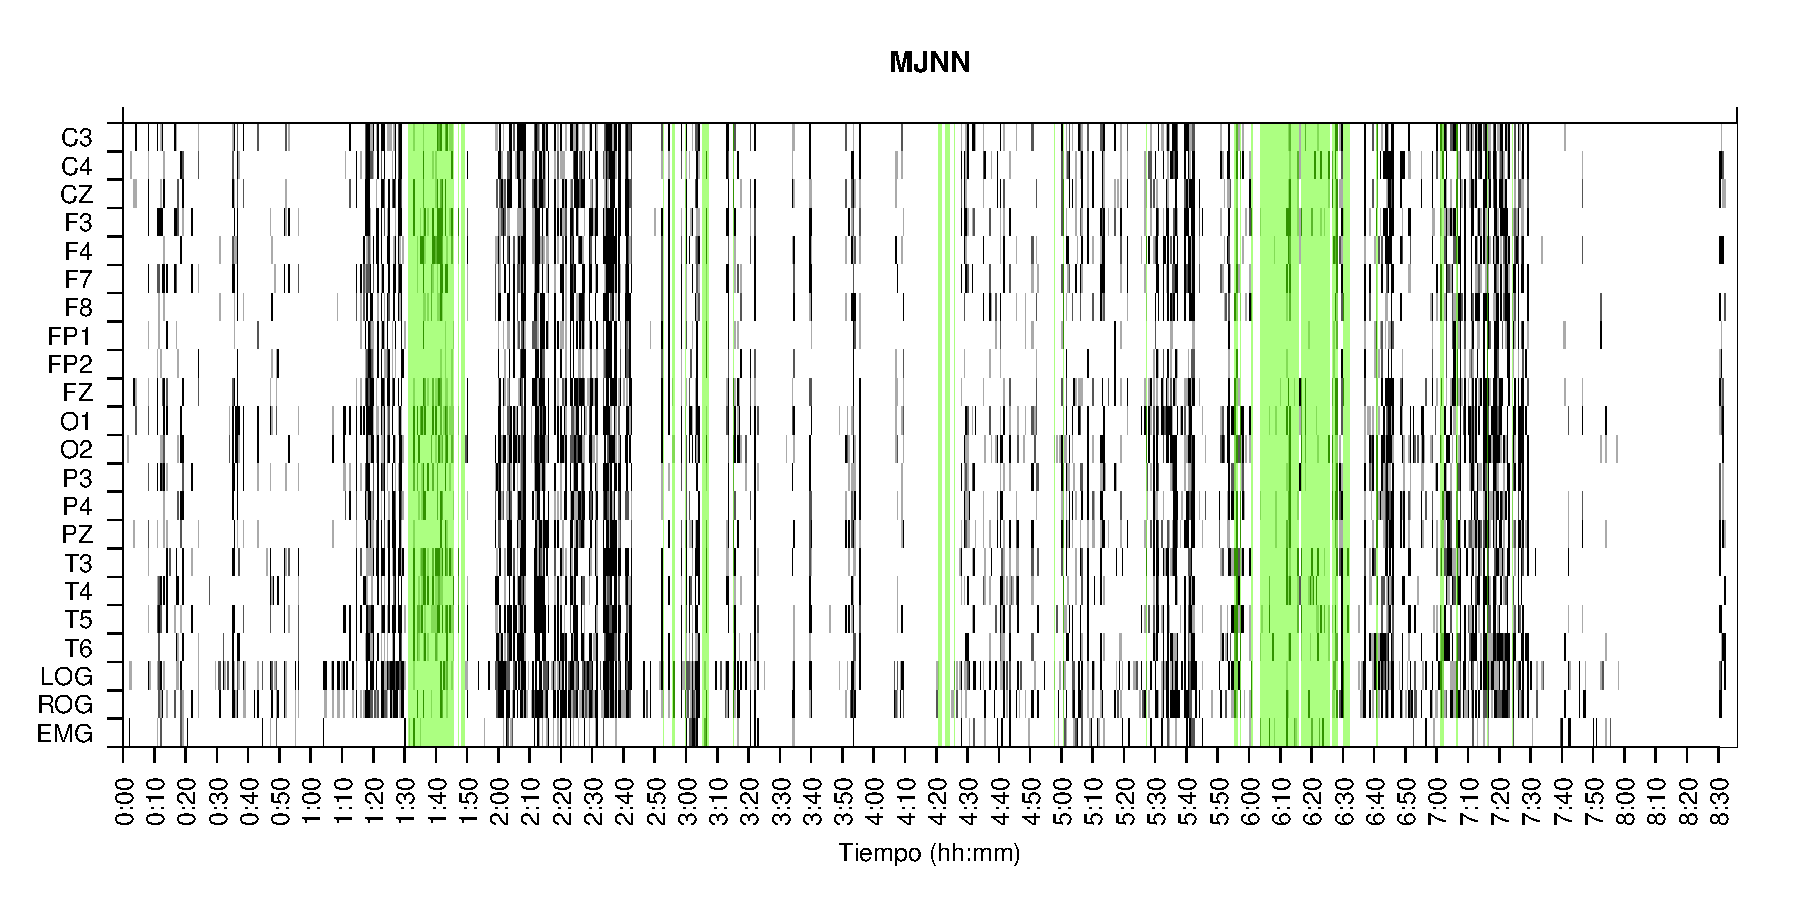
\includegraphics[width=\textwidth]{MJNNVIGILOS_127_mor127_tot1032_esttotal.pdf} 
\caption{Disposici\'on gr\'afica para los resultados del test PSR en el sujeto MJNN, 
para 1032 \'epocas de sue\~no y 22 canales. 
En el eje horizontal se muestra el tiempo desde el inicio de registro, en el eje vertical se muestra al 
nombre del canal. 
Se han resaltado con color verde las \'epocas clasificadas como sue\~no MOR (ver texto), que son 127.
Para este gr\'afico se consider\'o con un p-valor cr\'itico de 0.01 para la hip\'otesis
de estacionariedad. Ver texto para m\'as detalles.}
\label{ejemplo1}
\end{figure}

%\begin{figure}
%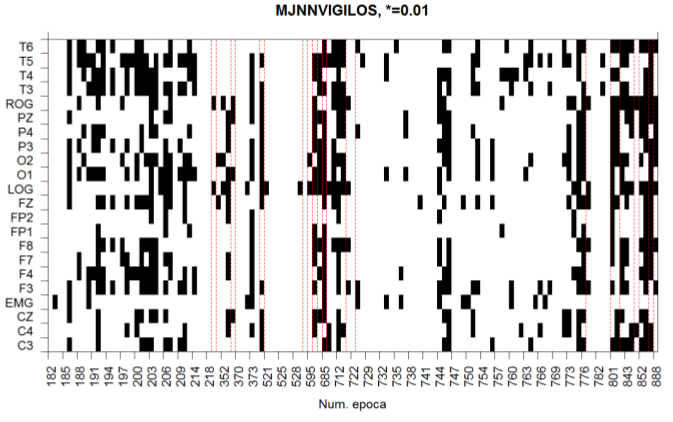
\includegraphics[width=\textwidth]{est02.png} 
%\caption{En este gráfico sólo se ilustran épocas MOR. Las líneas punteadas separan bloques continuos.
%Total de épocas: 1032 , Épocas MOR: 127}
%\label{ejemplo2}
%\end{figure}

%%%%%%%%%%%%%%%%%%%%%%%%%%%%%%%%%%%%%%%%%%%%%%%%%%%%%%%%%%%%%%%%%%%%%%%%%%%%%%%%%%%%%%%%%%%%%%%%%%%
%%%%%%%%%%%%%%%%%%%%%%%%%%%%%%%%%%%%%%%%%%%%%%%%%%%%%%%%%%%%%%%%%%%%%%%%%%%%%%%%%%%%%%%%%%%%%%%%%%%